\section{目的}
依據 PDF 81--84 頁重建 Lab 20，分開定義組合邏輯 propagation delay、輸出轉換時間及循序電路 setup/hold；以掃描得到成功／失敗邊界。

\section{Spec 對照}
S 表示已執行模擬檢查，D 表示分析與討論。

\small\begin{longtable}{p{.46\linewidth}p{.30\linewidth}p{.15\linewidth}}\toprule
要求與 PDF 頁碼 & 對應 deck／檢查 & 狀態 \\ \midrule\endhead
四級inverter、10fF及tr/tf/tPLH/tPHL（81,84） & D01/C0 & S \\
靜態DFF兩種資料setup（82--83） & D02; 62 cases & S \\
兩種資料hold及0時間案例（83） & D03; 102 cases & S \\
極短脈衝通過多級inverter（84） & D01/C1--5 & S \\
minimum pulse/release定義（84） & Discussion & D \\
\bottomrule\end{longtable}\normalsize


\section{電路與設計推導}
四級 inverter 使用 $W_p/W_n/L=3.6/1.8/0.25\,\mu$m，最後負載 10 fF。靜態 DFF 依圖20.2(b)以四個 transmission gate 和四個 inverter 組成 master/slave，輸出另接 10 fF。Master 於低時脈透明、slave 於高時脈透明，所以為正緣觸發。兩相時脈理想互補以分離本體 timing，沒有把反相器 clock skew 混入本次邊界。
\[t_{PLH/PHL}=t_{out,50\%}-t_{in,50\%},\quad t_r=t_{90\%}-t_{10\%},\quad t_f=t_{10\%}-t_{90\%}.\]
Setup offset 是資料50\%比clock50\%提早多少；hold offset 是資料50\%比clock50\%晚多少。負 hold 表示本測試中資料可在時脈50\%之前改變，不能直接解讀為任意時脈可提早改資料。

\section{模擬設定}
模型由使用者於本機另行提供；採 1 V、27 $^\circ$C 的教學適配條件，不把講義舊製程的 2.5 V 數值視為本次通過門檻。使用 PrimeSim HSPICE S-2021.09、\texttt{accurate}、\texttt{runlvl=5}，由實際 \texttt{.print/.measure} 數據繪圖。每個 \texttt{.alter} 重設全部基準參數與溫度。所有案例皆完成，無 error 或 failed 量測；這不代表完全沒有模型或收斂提示。公開 netlist 僅保留 \texttt{* MODEL\_SETUP\_REQUIRED} 註解，不附模型路徑。完整數據位於該 lab 的 \texttt{results/}，大型資料依 deck 分檔，由 \texttt{simulation\_data.json} 索引。三份 deck 共170案例。組合輸入邊緣5 ps，pulse width為1 ns及100/50/20/10/5 ps，最大步距0.5 ps。DFF時脈與資料邊緣20 ps，clock50\%在1.01 ns；setup掃-100至200 ps、hold掃-300至200 ps，步距10 ps，兩種資料極性皆測。DFF最大步距1 ps、總3.5 ns；在1.8 ns及3.0 ns分別檢查capture與保持，兩點皆達logic0 $\le0.1$ V或logic1 $\ge0.9$ V才通過。

\section{結果與規格檢查}
\begin{center}\small\begin{tabular}{lrrrrr}\toprule
Width (ps) & $V_{out,pk}$ (V) & $t_{PLH}$ (ps) & $t_{PHL}$ (ps) & $t_r$ (ps) & $t_f$ (ps) \\ \midrule
1000 & 1.1171 & 269.43 & 310.50 & 87.92 & 44.24 \\
100 & 0.7882 & 262.33 & 233.49 & -- & -- \\
50 & 0.0089 & -- & -- & -- & -- \\
20 & 0.0046 & -- & -- & -- & -- \\
10 & 0.0046 & -- & -- & -- & -- \\
5 & 0.0046 & -- & -- & -- & -- \\
\bottomrule\end{tabular}\end{center}

\begin{figure}[htbp]\centering
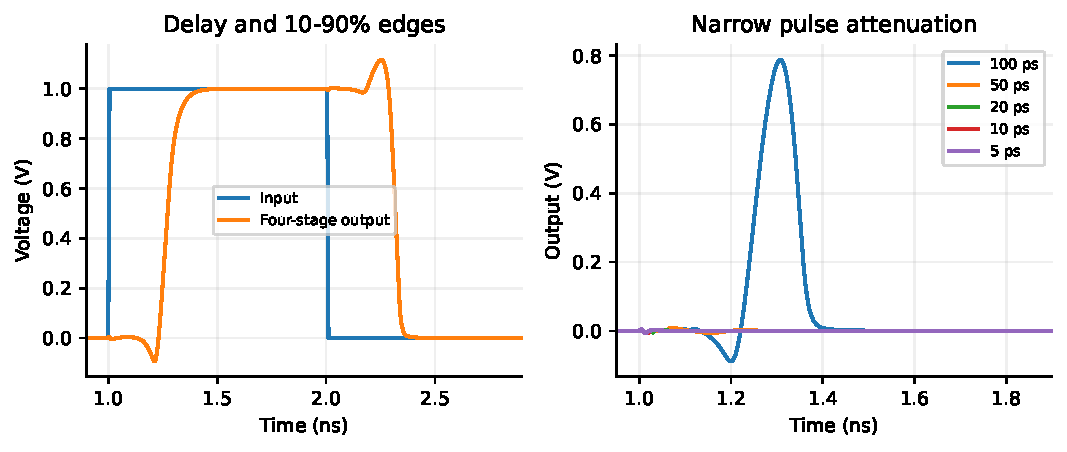
\includegraphics[width=\linewidth]{figures/chain_timing.pdf}
\caption{四級延遲與窄脈衝衰減。真實的過衝／下衝均保留。}
\end{figure}
\begin{center}\small\begin{tabular}{lrrr}\toprule
Check & Captured bit & Failing offset (ps) & Passing offset (ps) \\ \midrule
setup & 0 & 140 & 150 \\
setup & 1 & 110 & 120 \\
hold & 0 & -120 & -110 \\
hold & 1 & -150 & -140 \\
\bottomrule\end{tabular}\end{center}

\begin{figure}[htbp]\centering
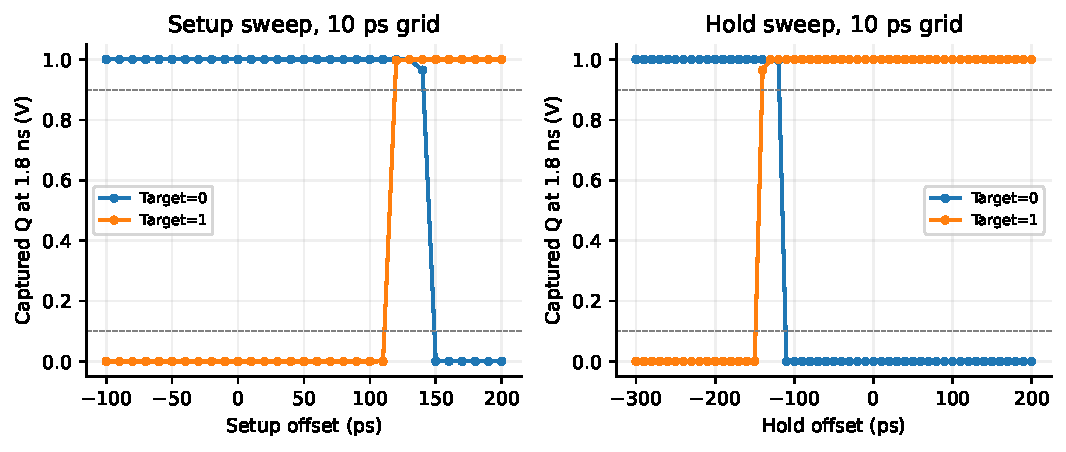
\includegraphics[width=\linewidth]{figures/dff_boundaries.pdf}
\caption{兩種極性的capture電壓隨offset變化。表中的判定還包含3.0 ns保持檢查。}
\end{figure}
本條件下最壞setup的通過點為150 ps，前一點140 ps失敗；另一極性為120 ps／110 ps。最保守hold通過點為-110 ps，前一點-120 ps失敗；另一極性為-140 ps／-150 ps。兩種極性在0 ps hold皆通過。這是10 ps網格與指定判準的界限，不是連續時間精確值或clock-to-Q退化型library規格。

100 ps脈衝仍達0.788 V但不達0.9 V有效高準位；50 ps以下沒有到達50\%的有效輸出脈衝。--代表該threshold crossing未出現，不是零延遲。

\section{討論}
多級inverter具有限頻寬與慣性，脈衝太窄時內部節點尚未充到切換門檻便反向，因此脈衝縮小或消失；接近門檻時可能仍出現不完整電壓而不能當乾淨數位訊號。此模型在快速理想源下有超軌暫態，未將它裁切或宣稱其符合可靠度額定。

Minimum pulse width是完成特定clock或set/reset功能所需的最小有效高／低脈寬；release/recovery time是非同步控制解除到有效clock緣間的最小間隔。圖20.2(b)沒有非同步set/reset腳，所以本報告解釋這兩個定義，沒有虛構對應控制腳的量測。Setup與hold互相關聯；本次分開掃描、其餘條件固定，不代表完整二維timing surface、PVT或metastability MTBF。

\section{結論}
講義要求的組合時序、雙極性setup/hold及窄脈衝問題都有實際結果。最壞setup通過點150 ps、hold=-110 ps適用於指定時脈、負載、模型與判準。
